\chapter{Research Objectives}

\section{Overall Goal and Approach}
Our overall goal is to investigate the feasibility of increasing children with ASD's engagement, prompt compliance, and task completion during COACH prompting for hand-washing tasks.  Our approach is to incorporate a half body humanoid robot, NAO T14 (see Figure \ref{fig:HalfBodyNAO}) by Aldebaran Robotics, into the current COACH setup, capable of delivering verbal and gesture prompts and attention grabbers.
%%\item to automatically track the VFOA of the child so that the robot can call out the child's name with a waving gesture or blink its LEDs for getting child's attention if the child is not looking at the robot before prompting

\begin{figure} [h]
	\centering
	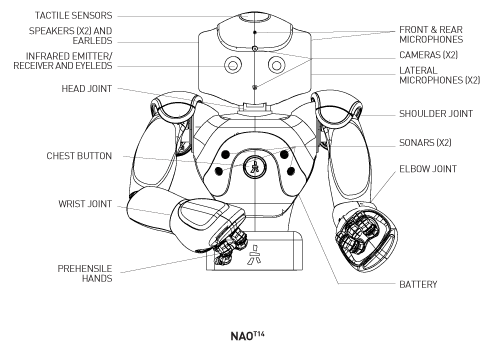
\includegraphics[width=0.6\textwidth]{./img/nao_t14_schema}
	\caption{The Half-Body Version of Humanoid Robot NAO}
	\label{fig:HalfBodyNAO}
\end{figure}


\section{Central Hypothesis}
We hypothesize that through the incorporation of a humanoid robot prompting agent, such as NAO T14, we would be able to show feasibility in better capturing and maintaining children with ASD's attention during prompting and keeping them engaged during task execution, so that high prompt compliance rates and task completion rates would be achieved when assisting them through ADLs such as hand-washing.


\section{Specific Objectives}

\paragraph{Our objectives are:}
\begin{enumerate}
	\item To investigate the feasibility of a prompting system using NAO to guide a child with ASD through hand-washing, and identify factors for improvement
	
	\item To explore the different modes of interactions between NAO and the child when prompting hand-washing steps using a Wizard of Oz setup, focusing on verbal, gestures, and gaze for the modes of interactions
	
%%	\item To explore how to implement a real-time algorithm for tracking child's VFOA
\end{enumerate}



\paragraph{Our hypotheses are:}

%	\item Child has greater general engagement level when interacting with NAO than with the parent.


%general engagement level:
%# of times child smiles
%# of times child murmurs
%# of times distracted

%visual focus correct:
%look at prompting agent given prompt rate
%look at step attempted given attempt rate

%prompt compliance and task completion:
%compliance rate
%# of prompts till compliance
%time duration till compliance
%task completion rate
%# of prompts till finished step before prompt
%time duration of extended steps
%number of presses for soap
%# of times requiring physical intervention

%independence:
%# of times child start step before prompt
%# of times child finishes step before prompt

%what measures for survey? just qualitative report? any processing / analysis needed before reporting?

\begin{enumerate}
	\item The humanoid robot, NAO, is able to demonstrate preliminary success in independently assisting child with ASD through hand-washing, and the child exhibits similar engagement level, complied prompt rate, and task completion when prompted by NAO as compared to when prompted by parent.
	
	\item Gestural, gaze, and verbal are the essential modes of interactions present in the hand-washing prompting scenario between child with ASD and the prompting agent NAO.
	
%	\item Using 3DMM and ALR for estimating head pose and eye pose, and using the Kinect camera, a classification rate of more than 80\% is achieved for estimating child's VFOA on NAO, monitor screen, soap, towel, tap region, hands, and idling.
	
\end{enumerate}
